\section{A code fragment analysis}
\label{sec:analysis}

\subsection{Syntax error and warning fixing}
First of all (although \textit{flawfinder} can analyse files that cannot even be compiled), inspecting the original code fragment (see subsection \ref{app:A}), trying to compile it and fixing possible typos/syntax errors, is good practice before (actually, after as well) analysing software:

\begin{description}[itemsep=1.5pt]
    \item[warnings at lines 3, 4, 5, 6:] extra tokens at end of \#include directive $\xrightarrow{fix}$ the extra ';' tokens are removed at the end of each line;
    \item[warning at line 26] implicit declaration of function 'read'; did you mean 'fread'? $\xrightarrow{fix}$ the missing \#include directive for 'unistd.h'\parencite{unistd.h} is added;
    \item[error at line 27] 'buf' undeclared (first use in this function); did you mean 'buf2'? $\xrightarrow{fix}$ the suggested correction is applied;
    \item[warning at line 39:] implicit declaration of function 'error'; did you mean 'perror'? $\xrightarrow{fix}$ 'error' is reasonably replaced by 'fprintf'\parencite{fprintf} rather than by 'perror'\parencite{perror}, since 'errno'\parencite{errno} is not set;
    \item[error at line 54:] expected '\{' at end of input $\xrightarrow{fix}$ the missing '\{' at the end of line 47 is added;
    \item[warnings at line 55:] implicit declaration of function 'len' [-Wimplicit-function-declaration] $\xrightarrow{fix}$ 'len' is reasonably replaced by 'strlen'\parencite{strlen}; passing argument 1 of 'strlen' makes pointer from integer without a cast $\xrightarrow{fix}$ 'foo' is passed as the first argument of 'strlen' instead of '*foo'.
\end{description}
Please note that, with respect to the request to run \textit{flawfinder} before fixing typos, these fixes do not have a significant impact on the analysis performed.

\subsection{Security warning analysis}
Now, running \textit{flawfinder} on the "preprocessed" code fragment (see subsection \ref{app:B}) using the flag '-m 0' or '--minlevel=0', to set the minimum risk level to 0 (i.e., the minimum risk level can go from 0 - "no risk" - to 5 - "maximum risk" - and the default is 1) for inclusion in the hitlist (i.e., final results), carries out the analysis results.

The analysis summary shows that there are some possible security vulnerabilities in the code fragment, as can be seen from figure \ref{fig:analysis_summary}.

\begin{figure}[H]
    \centering
    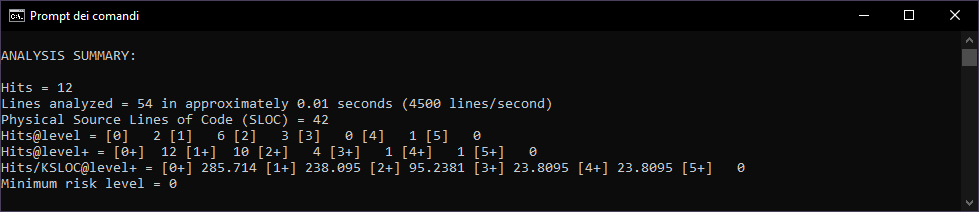
\includegraphics[width=0.9\textwidth]{Resources/analysis_summary.PNG}
    \caption{summary of the analysis of the code fragment (subsection \ref{app:B})}
    \label{fig:analysis_summary}
\end{figure}

In particular, the hits shown in the final results are twelve (mainly related to strings and buffer overflows), as can be seen from figure \ref{fig:final_results}:
\begin{description}[itemsep=1.5pt]
    \item[1) hit at line 52 (CWE-120\parencite{cwe-120}):] since the destination string 'buffer' is not large enough to receive the copy of the source string 'foo' the 'strcpy'\parencite{strcpy} invocation at line 52 will cause a buffer overflow, hence this hit is a vulnerability;
    \item[2) hit at line 10 (CWE-119!\parencite{cwe-119}/CWE-120):] since at line 13 'fgets'\parencite{fgets} is used to initialize 'buffer' and the second argument is set to the size in characters of 'buffer', 'buffer' will contain at most 1023 characters from 'stdin'\parencite{stdin} input channel (moreover, its 1024-th character will be the null byte), hence this hit is not a vulnerability (namely, 'buffer' is not improperly restricted);
    \item[3) hit at line 16 (CWE-119!/CWE-120):] since the destination string 'errormsg' is large enough to either receive the copy of the source string 'buffer' ('strncpy'\parencite{strncpy} at line 18) and to have the source string 'buffer' concatenated to itself ('strcat'\parencite{strcat} at line 19), and 'buffer' is null-terminated (by 'fgets' at line 13), this hit is not a vulnerability (namely, 'errormsg' is not improperly restricted) - moreover, 'errormsg' will be even null-terminated by 'strcat';
    \item[(4) hit at line 19 (CWE-120):] since 'errormsg' is large enough to store the result carried out by the invocation of 'strcat' at line 19, this hit is not a vulnerability;
    \item[(5) hit at line 18 (CWE-120):] since 'buffer' is null-terminated, after the 'strncpy' invocation at line 18, 'errormsg' will be null-terminated too, hence this hit is not a vulnerability;
    \item[6) hit at line 27 (CWE-120, CWE-20\parencite{cwe-20}):] since the third argument of 'read'\parencite{read} at line 27 is set to the size in bytes of 'len', this hit is not a vulnerability;
    \item[7) hit at line 29 (CWE-120, CWE-20):] since the third argument of 'read' at line 29 is set to the size (minus one) in characters (here, equal to the size in bytes minus one) of 'buf2', this hit is not a vulnerability;
    \item[8) hit at line 37 (CWE-120, CWE-20):] since the third argument of 'read' at line 37 is set to the size in bytes of 'buf3', this hit is not a vulnerability;
    \item[9) hit at line 45 (CWE-120, CWE-20):] since the third argument of 'read' at line 29 is set to the size in characters (here, equal to the size in bytes) of 'buf3', (yet 'buf3' will not be null-terminated in general: contrariwise, 'buf2' in 'func2' is explictly null-terminated at line 30), this hit is not a vulnerability (although all char buffers should be null-terminated);
    \item[10) hit at line 54 (CWE-126\parencite{cwe-126}):] since 'foo' is null-terminated by definition (even though the last character assigned to it is not explicitly the null byte, 'foo' is automatically null-terminated after being declared at line 49), this hit is not a vulnerability (namely, 'strlen' will not perform an over read);
    \item[11) hit at line 12 (CWE-134\parencite{cwe-134}):] since the format string passed as argument to 'printf'\parencite{printf} invocation at line 12 is constant, this hit is not a vulnerability (namely, no attacker can influence this format string);
    \item[12) hit at line 40 (CWE-134):] since the format string passed as argument to 'fprintf' invocation at line 40 is constant, this hit is not a vulnerability (namely, no attacker can influence this format string).
\end{description}

\begin{figure}[H]
    \centering
    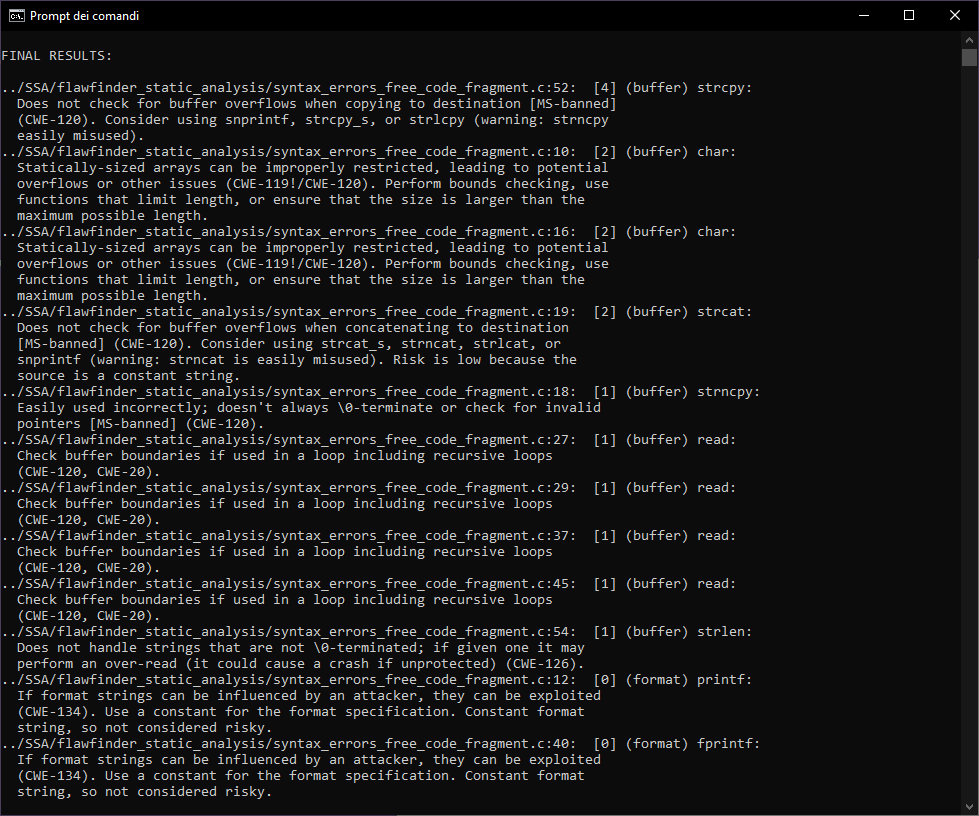
\includegraphics[width=0.9\textwidth]{Resources/final_results.PNG}
    \caption{final results of the analysis of the code fragment (subsection \ref{app:B})}
    \label{fig:final_results}
\end{figure}


\subsection{Other vulnerabilities and flaws}
Inspecting code again might help find other security vulnerabilities or simply weaknesses.

For instance, the following should be considered:
\begin{description}[itemsep=1.5pt]
    \item[return value checking:] with respect to each function invocation in the code, return values (if present) should be checked to determine whether a function (e.g., 'printf', 'fgets', 'malloc'\parencite{malloc}, 'read', \ldots) has been successfully executed or not;
    \item[exit in case of error:] when an error is detected it should be handled (e.g., terminating the code execution or trying again);
    \item[unsafe string library usage:] since some standard string library (i.e., 'string.h'\parencite{string.h}) functions (e.g., 'strcpy', \ldots) have been banned and have more robust or secure replacements (i.e., these functions are deprecated), a safe string library should be used instead (e.g., 'strsafe.h'\parencite{strsafe.h});
    \item[memory management:] with respect to memory allocation, 'calloc'\parencite{calloc} might be used rather than 'malloc' (e.g., to zero out memory in advance), furthermore allocated memory should be eventually released using 'free'\parencite{free};
    \item[explicit type casting:] when useful (e.g., 'calloc' return value, for code readability or disambiguation) or required (e.g., 'isalpha'\parencite{isalpha} checks argument to have the value of an
       unsigned char or EOF) explicit type conversion should be performed.
\end{description}